%%%%%%%%%%%%%%%%%%%%%%%%%%%%%% -*- Mode: Latex -*- %%%%%%%%%%%%%%%%%%%%%%%%%%%%
%% project-researchplan.tex -- 
%% Author          : Philip Johnson
%% Created On      : Thu Oct  4 08:05:31 2001
%% Last Modified By: Philip M. Johnson
%% Last Modified On: Thu May 26 08:41:40 2005
%% RCS: $Id$
%%%%%%%%%%%%%%%%%%%%%%%%%%%%%%%%%%%%%%%%%%%%%%%%%%%%%%%%%%%%%%%%%%%%%%%%%%%%%%%
%%   Copyright (C) 2001 Philip Johnson
%%%%%%%%%%%%%%%%%%%%%%%%%%%%%%%%%%%%%%%%%%%%%%%%%%%%%%%%%%%%%%%%%%%%%%%%%%%%%%%
%% 

\section{Research Plan}

We begin by presenting our research plan as three high-level initiatives:
the design, implementation, and evaluation of the Cedar infrastructure.  We
then present a more low-level view of the plan in terms of tasks,
milestones, coordination activities, outreach, and dissemination.

\subsection{Design of Cedar}

Section \ref{sec:cedar} summarized the high level requirements for the
Cedar system: an open source information infrastructure architecture
coupled with a data management policy mechanism that supports scalable and
collaborative, qualitative and quantitative organizational research data
collection, analysis, dissemination, and archiving.  The risk level
associated with each requirement varies according to whether it
necessitates advances in the state of the art.  A primary goal of the Cedar
design phase is to focus on the high risk requirements and perform the
research necessary to reduce the level of risk associated with them.  In
this project, risk assessment, risk reduction, and system design is an
ongoing, iterative activity. We have identified three design issues for
initial risk reduction: privacy policies, repository data management, and
representational support for qualitative and quantitative data integration.

{\bf Design of privacy policies.} There is an inherent tension between privacy and
utility with respect to empirical data.  The more you know about the data
and the context under which it was collected, the more likely you are to
assign a meaning or interpretation to the data that aids in understanding
and/or decision-making. At the same time, the more you know about the data,
the less privacy exists with respect to the individuals and organizations
associated with it.  We do not expect to eliminate this tension in the
design of Cedar, but rather to leverage our own prior experience and other
research to invent better mechanisms to manage this tension between privacy
and utility.  For example, traditional empirical data privacy policies are
neither context-sensitive nor time-dependent: a subject signs a consent
form that specifies a single type of access by a single type of researcher
which never changes.  A cyberinfrastructure for empirical data enables a
more flexible approach in which a subject could specify different levels of
privacy for different groups of people.  Furthermore, the desired privacy
could evolve over time: an organization might require high levels of
privacy for data associated with a product under current development, but
might be willing to loosen privacy levels a decade later after the product
has been retired.  PI Johnson will lead this design effort.

{\bf Design of repository data management.}  Prior experience by both PI Basili and
PI Johnson with public empirical data repositories indicate that ``if you
build it, they will come.''  However, many important issues remain: how can
we help ensure that ``they'' use the data appropriately? How can we create
appropriate incentives so that ``they'' want to contribute new data as well
as extract insight from the old?  How can we create a self-sufficient
repository that supports the ongoing need for hardware, software, and
technical support resources?  PI Basili will lead this design effort as a
natural extension of his ongoing leadership role in the software
engineering task force on data repositories.

{\bf Design of narrative and network representation for integration of
qualitative and quantitative data.}  Prior research by PI Pentland and PI
Feldman indicate that narrative and network representations show great
promise as a means to integrate qualitative and quantitative data,
providing the context and etic/emic perspectives necessary to derive
meaning from data.  For example, both qualitative and quantitative data in
Cedar could be indexed using categories from narrative analysis, such as
Burke's grammar of motives (actor, act, scene, agency, purpose) or
Fillmore's case grammar \cite{Burke69,Fillmore68}. The choice of exactly
which dimension to include, and the extent to which customization is
allowed, are important research questions.  For example, we can add
additional elements to the structure, such as ``input'' and ``output'', so
that we could support generic process representations, such as the Process
Specification Language (PSL).  Questionnaires, surveys, spatial coordinates
or other properties (e.g., generic keywords) could also be added when
necessary, without loss of generality for the basic indexing mechanism.  PI
Pentland has data on customer service processes in Citibank that can be
used to support initial design and risk reduction.  PI Pentland and PI
Feldman will lead this design effort.

\subsection{Implementation of Cedar}

The Cedar implementation, and the process we use to achieve it, will be
modeled in many ways on the Hackystat Project.  Hackystat already embodies
many of the attributes we need for Cedar, and we can leverage our
experiences with the Hackystat development process and the software that
has resulted to jump-start Cedar development.  Hackystat has gone through
five major architectural revisions since its inception, as we worked
through issues related to scalability, extensibility, and configurability,
and currently consists of approximately 100,000 lines of code.  The current
architecture enables us to implement both a generic infrastructure for
collection and analysis of quantitative software engineering data, as well
as a set of ``configurations'', or enhancements to this generic
infrastructure that customize the data collected and the way it is analyzed
to the needs of a specific situation.  The Hackystat project is
self-instrumented, and we use measurements of our own process and products
to maintain a balance between quality assurance and enhancement activities.

The requirements for Cedar will require three major extensions to
Hackystat: a federated peer-to-peer network of servers; support for
qualitative data collection and storage; and an enhanced client-side user
interface.

{\bf Federated servers.}  Hackystat implements a fairly standard
client-server architecture: sensors collect data from client systems and
sends it to a Hackystat server for storage and analysis.  We maintain a
public Hackystat server to which anyone can send data, though some
organizations prefer to install and maintain their own server so that data
about their processes and products remains internal.  Cedar
will extend this basic paradigm by allowing servers to establish
communication with each other, creating a federated, peer-to-peer network
of Cedar servers. This architecture will have an interesting impact on the
design of privacy policies: it seems likely that a user will wish to
establish both a ``local'' privacy policy (i.e. for how their data is
protected in the server where it is physically located) and a ``global''
privacy policy (i.e. for how their data might be disseminated upon request
to other servers.)

{\bf Qualitative data collection and storage.} Hackystat does not currently
collect or store qualitative data.  Cedar will extend support to collection
and storage of many, but not all, forms of qualitative data.  Cedar will
not, for example, provide the ability for users to upload a digital version
of a feature film and store it along with indexes into various scenes of
interest.  Such kinds of qualitative data must be represented in Cedar
indirectly: instead of storing the actual file containing the feature film,
Cedar might store, for example, an URL to a location on the internet
containing the film, along with information describing how to access the
scenes of interest using some appropriate viewer.

{\bf User interface.} Hackystat's user interface is web-based, consisting
of HTML forms for entry of information and static tabular or chart data as
the results of analyses.  The advantage of a web-based interface is that
users with only a browser can access and manipulate Hackystat services.
The disadvantage is the constraints that HTML places on the way data is
entered, displayed, and manipulated.  For Cedar, we will design and
implement a more sophisticated client-side application called CedarView
that will allow display, entry, and analysis of both qualitative and
quantitative information.  CedarView will be inspired by multi-track
editors for music, such as Apple's GarageBand.  Upon execution, CedarView
will connect to one or more Cedar servers, download the appropriate data,
and display it as a series of ``tracks'' organized along a timeline.  It
will allow the user to ``zoom in'' or ``zoom out'' of the chosen data
streams, and ``cut and paste'' data streams from one timeline to
another. It will allow annotation of timelines with additional information,
such as for encoding episodes with classifiers. Finally, CedarView will be
extensible through a plug-in architecture to support processing of the raw
data in various ways.  For example, one plug-in might produce a timed
markov model, while another might produce a social network representation.

\subsection{Evaluation of Cedar}

Evaluation of Cedar will be an ongoing process throughout the project,
where the artifacts to be evaluated and the approach to be used will depend
upon the stage of development of the system.  For example, early in the
project, we will seek community review and evaluation of design documents
regarding our approach to privacy policies, repository data management, and
the representation and integration of qualititative and quantitative data.
To facilitate this evaluation, we will form an advisory board from a
variety of academic and industrial disciplines to ensure broad perspectives
and feedback on our approach. 

As elements of the Cedar infrastructure come online, we will begin a series
of evaluative case studies to assess how well the infrastructure is
fulfilling its requirements.  We will begin with classroom use to assess
basic functionality and usability.  After this use indicates sufficient
stability and functionality, we plan to incrementally deploy Cedar into the
High Productivity Computing Systems organization, as described in Section
\ref{sec:motivation}.

Case studies in the HPCS organization will allow us to ``stress-test''
virtually all of functionality intended for Cedar.  As a distributed
organization, use of Cedar by HPCS will naturally lead to a set of
intercommunicating servers.  The relationships between the various
organizations will test the ability of our privacy policies to enable
sharing of data while providing adequate protection to the subjects and
organizations who generated it.  The diversity of qualitative and
quantitative data will test the ability of Cedar to represent this
information and make useful connections between them.  Finally, the
national importance of the HPCS program and the level of commercial and
government investment in it provides natural incentives for long-term
resources for management of the Cedar repository, and tests the abilities
of our management policies to exploit those potential resources.

Use of Cedar in the HPCS domain will provide a body of experiences, data,
and technology transfer insights that we will exploit to gain insight into
the requirements for broader outreach and dissemination of this technology
to the scientific community.  We anticipate forming a ``Cedar Consortium''
of academic and commercial organizations, along with a yearly users group
meeting to share experiences and develop plans for future growth.  The
Apache and Eclipse communities provide models for how the various legal,
organizational, and development issues can be resolved to form a vibrant
community of users and developers.

\subsection{Coordination plan, timeline, outreach, and dissemination}


\begin{figure*}[ht]
  \centering
  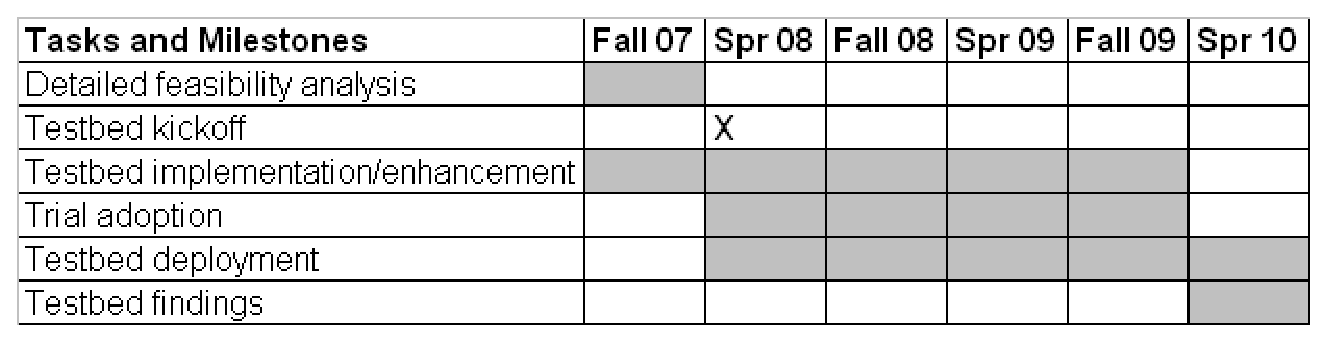
\includegraphics[width=0.75\textwidth]{workstructure.eps}
  \caption{Work breakdown structure and milestones}
  \label{fig:timeline}
\end{figure*}

Figure \ref{fig:timeline} outlines the major tasks, lead PI(s), and
milestones we have planned for this project.  Although all PIs will be in
close communication and involved with all aspects of the project, we
believe that some decoupling, particularly in the initial phase of the
project, will enable us to make progress more quickly.  

In the initial year, the primary tasks will be to design privacy policies,
narrative/network representations, and data repository management
mechanisms; and implement the architectural framework for Cedar. We will
also perform some ``pre-pilot'' case study work to validate our current
requirements and gather additional ones for deployment of Cedar into the
HPCS organization.  At the end of this initial year, we will make a public
release of our framework along with documents specifying the results of our
design activities.

In the second year, we will implement the designs developed during the
first year, and begin classroom case studies with Cedar which will result
in curriculum materials.  By half way through the funding period, at the
beginning of the third year, we plan to have a first release of the fully
functional Cedar cyberinfrastructure.

While we plan to continuously refine and improve the system for the
remainder of the grant period, this process will be driven by more
comprehensive evaluation activities during the second half of the grant
period, including pilot courses, case studies in the HPCS organization, and
external evaluation.  In the final year, we will begin effort on technology
transfer, developing documentation and training materials and conducting
tutorials as necessary to help broaden usage of Cedar.  By the end of the
grant period, we plan for a federated network of at least 50 to 100 Cedar
servers in active use, and that the success of this framework in the HPCS
community has created interest and involvement in the Cedar Consortium by
both academic and commercial organizations.

All of the PIs have extensive prior experience working in distributed
``virtual'' organizations, and we have learned how to be productive despite
geographical separation.  We will use a variety of synchronous and
asynchronous mechanisms to facilitate communication and coordination among
the Cedar research group. We plan to have a weekly teleconference meeting
between the PIs and graduate students to discuss tasks and challenges. Our
travel budgets include funds for on-site meetings twice a year for more
intensive, face-to-face interaction where we can review progress and
establish goals and milestones for the next six month period.  Finally, we
will provide a website similar to www.hackystat.org that will provide a
portal for access to source code, documentation, tech reports, wiki
collaboration, a public Cedar server, and so forth.

\subsection{Cedar in action}

To illustrate the benefits of Cedar, consider once again Figures
\ref{fig:dailydiary} and \ref{fig:telemetry}, which illustrate some of
quantitative data available about a high performance computing system
development project.  Effective interpretation and application of this
experience raises many questions : Are the trends in serial and parallel
code typical? Under what circumstances would a new development project
produce the same size trends? What are the strengths and weaknesses of the
chosen tool set (g++, mpiCC, etc.)?  Answering these questions requires
contextual, qualitative data, much of which is potentially available in
other artifacts associated with this study (the developer's engineering
logs, emails, and so forth).

One goal of Cedar is to provide an effective representation for tying the
quantitative to the qualitative, and it accomplishes this by supporting the
creation of a high-level abstract narrative, or ``story'' of this
development project which incorporates both the quantitative numbers and
the explanations for how the numbers came about.  In this case, some of the
relevent context is that the developer is a graduate student, was
implementing his first MPI program, was more concerned with functional
correctness than parallel speedup during this project, and encountered a
major requirements change in February 2005, leading to the sudden
perturbation in both parallel and serial code size. Such context is crucial
for assigning meaning to these numbers.

The narrative representation has another benefit beyond data integration:
it also provides a way for a user to query the federated network of Cedar
servers for similar ``stories''.  For example, having constructed this
narrative, one can then query the network to learn about other case studies
involving, for example, MPI software development.  The level of detail
provided back in response to this query will depend upon the privacy
policies in force related to each instance of the narrative. The
incremental generation of a collection of narratives, related in various
ways, creates a rich web of qualitative and quantitative data that provides
context for each single narrative as part of a larger community of
practice.





















